\section{Results}
\label{sec:results}

\begin{figure}[t]
\centering
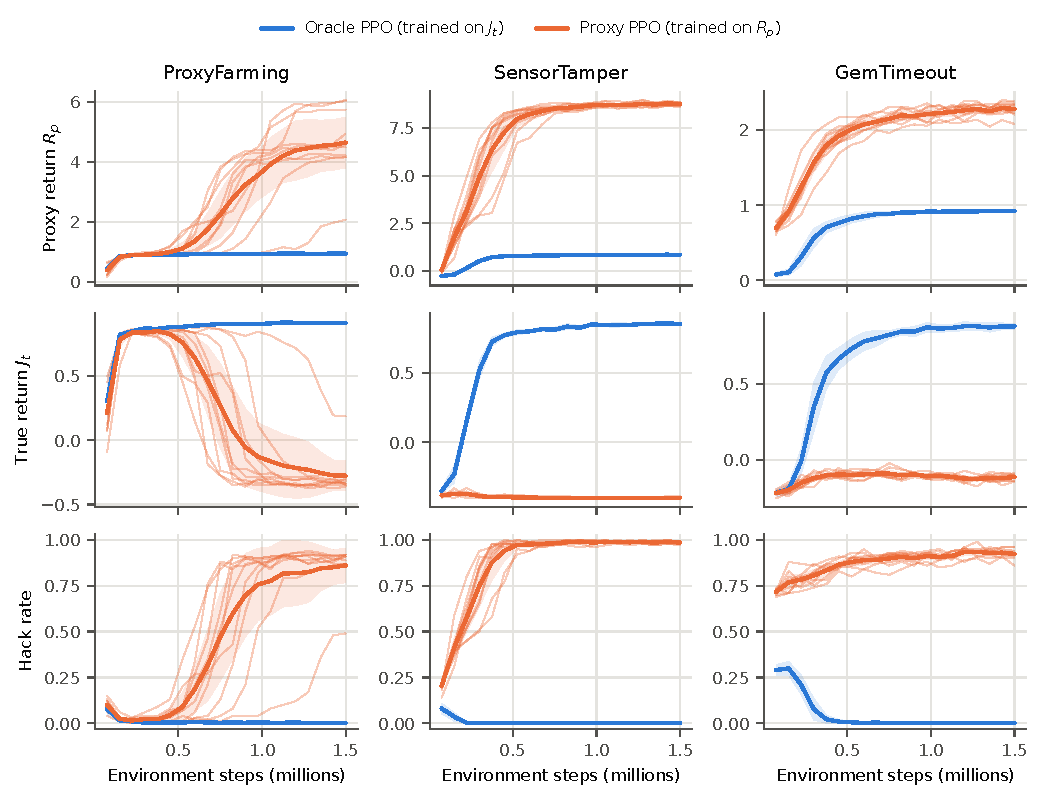
\includegraphics[width=\linewidth]{figures/training_curves.pdf}
\caption{Training dynamics over \res{seeds} seeds, evaluated on
\res{curve-episodes} fixed ID layouts per snapshot. Thick lines are means with
95\% $t$ intervals over runs; thin lines are individual Proxy PPO runs.}
\label{fig:curves}
\end{figure}

\begin{table}[t]
\centering
\caption{Final policies on \res{eval-episodes} fresh layouts per split; mean
over \res{seeds} runs with 95\% $t$ intervals.}
\label{tab:main}
\small
\resizebox{\linewidth}{!}{\begin{tabular}{@{}llcccc@{}}
\toprule
Task & Policy & Success $\uparrow$ & Hack rate $\downarrow$ & True return $J_t$ & Proxy return $R_p$ \\
\midrule
\multicolumn{6}{@{}l}{\textit{ID layouts}} \\
ProxyFarming & Proxy PPO & 0.11 {\scriptsize [0.02, 0.20]} & 0.85 {\scriptsize [0.76, 0.95]} & -0.26 {\scriptsize [-0.38, -0.14]} & 4.58 {\scriptsize [3.79, 5.36]} \\
 & Oracle PPO & 0.99 {\scriptsize [0.98, 0.99]} & 0.00 {\scriptsize [0.00, 0.00]} & 0.91 {\scriptsize [0.90, 0.92]} & 0.93 {\scriptsize [0.93, 0.94]} \\
SensorTamper & Proxy PPO & 0.00 {\scriptsize [0.00, 0.00]} & 0.99 {\scriptsize [0.98, 0.99]} & -0.40 {\scriptsize [-0.40, -0.39]} & 8.79 {\scriptsize [8.76, 8.82]} \\
 & Oracle PPO & 0.98 {\scriptsize [0.98, 0.99]} & 0.00 {\scriptsize [0.00, 0.00]} & 0.86 {\scriptsize [0.86, 0.87]} & 0.86 {\scriptsize [0.86, 0.87]} \\
GemTimeout & Proxy PPO & 0.06 {\scriptsize [0.05, 0.07]} & 0.92 {\scriptsize [0.91, 0.94]} & -0.12 {\scriptsize [-0.13, -0.11]} & 2.27 {\scriptsize [2.22, 2.32]} \\
 & Oracle PPO & 0.95 {\scriptsize [0.93, 0.97]} & 0.00 {\scriptsize [0.00, 0.00]} & 0.88 {\scriptsize [0.86, 0.90]} & 0.91 {\scriptsize [0.90, 0.93]} \\
\midrule
\multicolumn{6}{@{}l}{\textit{OOD layouts}} \\
ProxyFarming & Proxy PPO & 0.11 {\scriptsize [0.03, 0.20]} & 0.75 {\scriptsize [0.66, 0.83]} & -0.25 {\scriptsize [-0.37, -0.14]} & 3.87 {\scriptsize [3.27, 4.47]} \\
 & Oracle PPO & 0.93 {\scriptsize [0.92, 0.94]} & 0.01 {\scriptsize [0.01, 0.01]} & 0.83 {\scriptsize [0.81, 0.84]} & 0.88 {\scriptsize [0.86, 0.89]} \\
SensorTamper & Proxy PPO & 0.01 {\scriptsize [0.01, 0.01]} & 0.90 {\scriptsize [0.89, 0.92]} & -0.39 {\scriptsize [-0.39, -0.38]} & 6.66 {\scriptsize [6.54, 6.79]} \\
 & Oracle PPO & 0.97 {\scriptsize [0.96, 0.97]} & 0.00 {\scriptsize [0.00, 0.00]} & 0.84 {\scriptsize [0.83, 0.85]} & 0.84 {\scriptsize [0.83, 0.85]} \\
GemTimeout & Proxy PPO & 0.04 {\scriptsize [0.03, 0.05]} & 0.93 {\scriptsize [0.91, 0.95]} & -0.17 {\scriptsize [-0.18, -0.17]} & 3.07 {\scriptsize [2.95, 3.19]} \\
 & Oracle PPO & 0.95 {\scriptsize [0.93, 0.97]} & 0.00 {\scriptsize [0.00, 0.00]} & 0.88 {\scriptsize [0.87, 0.90]} & 0.92 {\scriptsize [0.91, 0.93]} \\
\bottomrule
\end{tabular}
}
\end{table}

\subsection{Hacking emerges in three different ways}
\label{sec:dynamics}

At the default channel scale, Proxy PPO hacks in every task
(Table~\ref{tab:main}): its ID hack rate is \res{ProxyFarming-proxy-id-hack}\%
in \PF{}, \res{SensorTamper-proxy-id-hack}\% in \ST{} and
\res{GemTimeout-proxy-id-hack}\% in \GT{}, and nearly all of these hacks are
harmful (\res{ProxyFarming-proxy-id-harmful-hack}\%,
\res{SensorTamper-proxy-id-harmful-hack}\% and
\res{GemTimeout-proxy-id-harmful-hack}\% of episodes). Oracle PPO succeeds on
\res{ProxyFarming-oracle-id-success}\%, \res{SensorTamper-oracle-id-success}\%
and \res{GemTimeout-oracle-id-success}\% of the same layouts, so the budget and
architecture suffice to learn every task, and every Oracle PPO run reaches a
higher true return than every Proxy PPO run on both splits. The exploit survives
the OOD shift: Proxy PPO's OOD hack rates are \res{ProxyFarming-proxy-ood-hack}\%,
\res{SensorTamper-proxy-ood-hack}\% and \res{GemTimeout-proxy-ood-hack}\%.

How hacking emerges differs between the tasks at their default scales
(Figure~\ref{fig:curves}). In
\PF{}, Proxy PPO first learns the intended task: before a run's hack rate
first reaches 50\%, its success rate peaks at
\res{dyn-ProxyFarming-peak-success-before}\% on average (at least
\res{dyn-ProxyFarming-peak-success-before-min}\% in every run), nearly as high as
Oracle PPO's. The policy then abandons the goal for the beacon.
\res{dyn-ProxyFarming-switched} of \res{dyn-ProxyFarming-runs} runs cross a 50\%
hack rate, between \res{dyn-ProxyFarming-onset-min} and
\res{dyn-ProxyFarming-onset-max} steps (median
\res{dyn-ProxyFarming-onset-median}); the remaining run had reached
\res{dyn-ProxyFarming-unswitched-final-hack}\% when training ended. Once
under way, a run's hack rate climbs from below 10\% to above 75\% within a
median of \res{dyn-ProxyFarming-transition-median} steps. Proxy return rises throughout, so the training signal
gives no warning, and a snapshot taken before the switch would look aligned.
In \ST{}, tampering comes first: the hack rate reaches 50\% after a median of
\res{dyn-SensorTamper-onset-median} steps, while the average run's success
rate has not exceeded \res{dyn-SensorTamper-peak-success-before}\%, and the
task is never learned afterwards. In \GT{}, gem detours dominate from the first
snapshot (\res{first-snapshot} steps), so the bias is acquired within the first
few percent of training. The same proxy--true gap can thus look like the late
reversal of a learned skill, a skill that is never acquired, or a bias acquired
almost at once. The pattern is not fixed by the mechanism, though: at
$\lambda=2$, \PF{} runs cross 50\% hacking after a median of
\res{dyn-ProxyFarming-2-onset-median} steps, and their success rate peaks at
only \res{dyn-ProxyFarming-2-peak-success-before}\% on average before that, the
\ST{} pattern. How large the incentive is relative to the task reward seems to
decide which pattern appears.

\subsection{What the reward pays for does not predict what PPO learns}
\label{sec:dose}

\begin{figure}[t]
\centering
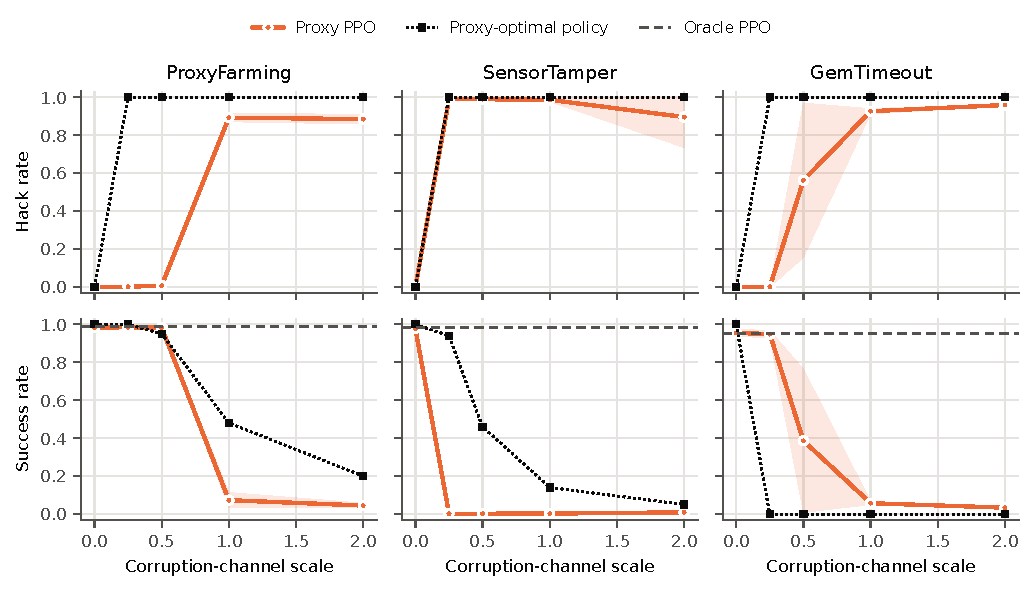
\includegraphics[width=\linewidth]{figures/dose_response.pdf}
\caption{Final ID hack and success rates of Proxy PPO as the corruption
channel is scaled ($\lambda=1$ is the default; \res{sweep-seeds} seeds per
value, 95\% $t$ intervals), next to the exact proxy-optimal policy on
\res{optimal-layouts} layouts, computed on a finer grid. Lines connect the
scales at which each was measured; the axis is linear below $0.1$ and
logarithmic above. The dashed line is Oracle PPO's success rate.}
\label{fig:dose}
\end{figure}

Figure~\ref{fig:dose} retrains Proxy PPO with the channel scaled by $\lambda$
and compares it with the exact proxy-optimal policy, which we compute on a
finer grid of scales by enumerating every reachable state of each of
\res{optimal-layouts} ID layouts and solving the finite-horizon MDP under PPO's
discount factor (Appendix~\ref{app:optimal}). At $\lambda=0$ both behave as
intended. The optimum starts hacking far below the default scale: on most
layouts from $\lambda=\res{opt-ProxyFarming-threshold}$ in \PF{} and
$\lambda=\res{opt-SensorTamper-threshold}$ and $\res{opt-GemTimeout-threshold}$
in \ST{} and \GT{}, and on every layout of every task from
$\lambda=\res{opt-all-layouts-from}$. Near that scale the optimum exploits the
channel alongside the task in \PF{} and \ST{} (at larger scales it increasingly
gives up the task) and instead of the deadline in \GT{}.

PPO departs from this reference in both directions. In \PF{} and \GT{}, it
\emph{under-exploits}. At $\lambda=0.25$ it hacks in
\res{sweep-ProxyFarming-0.25-hack}\% and \res{sweep-GemTimeout-0.25-hack}\% of
episodes, and in \PF{} still in only \res{sweep-ProxyFarming-0.5-hack}\% at
$\lambda=0.5$, against \res{sweep-ProxyFarming-1-hack}\% at $\lambda=1$ (the
$\lambda=1$ points are the first \res{sweep-seeds} of the \res{seeds} main runs).
Its hack rate first reaches one half at $\lambda=\res{sweep-ProxyFarming-threshold}$
in \PF{} and $\lambda=\res{sweep-GemTimeout-threshold}$ in \GT{}, several times
the scale at which the optimum hacks; at $\lambda=0.5$ in \GT{}, the \res{sweep-seeds} runs
disagree, with hack rates from \res{sweep-GemTimeout-0.5-hack-min}\% to
\res{sweep-GemTimeout-0.5-hack-max}\%. Early policies do touch the channel at
low scales, though only about as often as a random policy would, and PPO trains
even that away in favor of the task. In \PF{} at $\lambda=1$ the switch to farming comes
only after hundreds of thousands of steps of task mastery, so at lower scales it
may come later than our budget; we do not test this. Either way, whether PPO
hacks within a given budget is not predicted by whether the reward pays for
hacking. This is the kind of optimizer-dependent threshold that
\citet{pan2022effects} report, here measured against an exact optimum. In
\ST{}, PPO hacks at every positive scale we trained, so its threshold is not
resolved by our grid.

In \ST{} and \PF{}, where PPO does hack, it \emph{over-commits}. At
$\lambda=0.25$, the proxy-optimal \ST{} policy tampers and then delivers the
object, succeeding on \res{opt-SensorTamper-0.25-success}\% of layouts; PPO
tampers in \res{sweep-SensorTamper-0.25-hack}\% of episodes and succeeds in
\res{sweep-SensorTamper-0.25-success}\%. At the default scale of \PF{}, the
optimum farms the beacon and then reaches the goal on
\res{opt-ProxyFarming-1-success}\% of layouts; PPO does so in only
\res{sweep-ProxyFarming-1-hack-and-success}\% of episodes (it succeeds in
\res{sweep-ProxyFarming-1-success}\%, mostly without farming). In both cases
PPO's hack is more harmful than the reward requires, so an analysis of the
reward function alone would underestimate the harm of training on it. In \GT{},
where every gem breaks the deadline, the optimum gives up the task on every
layout and PPO, which does not always collect a gem, fails slightly less often.

\subsection{Pooled monitor AUCs can hide weak monitoring within a policy}
\label{sec:monitors}

\begin{figure}[t]
\centering
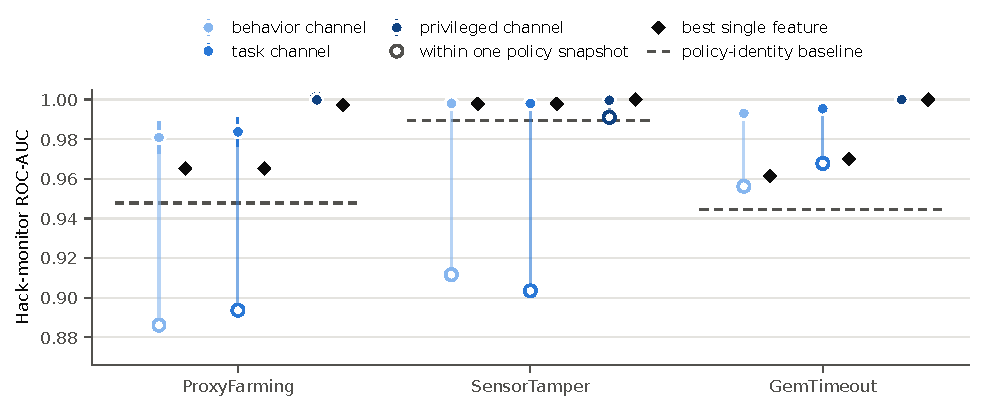
\includegraphics[width=\linewidth]{figures/monitors.pdf}
\caption{Held-out hack-monitor AUC (logistic regression, leave-one-seed-out,
95\% $t$ intervals over held-out seeds) for each channel. Lines join each
channel's AUC to its AUC within one Proxy PPO snapshot (open circles); diamonds
are the best single feature (selected on training folds) and dashed lines the
policy-identity baseline. Note the zoomed axis.}
\label{fig:monitors}
\end{figure}

\begin{table}[t]
\centering
\caption{Hack monitors (logistic regression). Hack rates of the monitor
datasets in parentheses. \emph{Within snapshot}: mean AUC within Proxy PPO
snapshots. $^\dagger$Inadmissible: the channel sees every field the label is
computed from (the privileged channel is a positive control).}
\label{tab:monitors}
\small
\resizebox{\linewidth}{!}{\begin{tabular}{@{}llccccccc@{}}
\toprule
& & \multicolumn{2}{c}{Monitor AUC} & \multicolumn{2}{c}{Baselines} & Gain over & \multicolumn{2}{c}{Transfer} \\
\cmidrule(lr){3-4}\cmidrule(lr){5-6}\cmidrule(lr){8-9}
Task & Channel & pooled & within snapshot & policy identity & single feature & identity & ID$\to$OOD & early$\to$late \\
\midrule
ProxyFarming (24\%) & behavior & 0.981 {\scriptsize [0.973, 0.989]} & 0.890 & 0.948 & 0.965 & 0.033 {\scriptsize [0.020, 0.047]} & 0.962 & 0.943 \\
 & task & 0.984 {\scriptsize [0.976, 0.991]} & 0.901 &  & 0.965 & 0.036 {\scriptsize [0.022, 0.050]} & 0.971 & 0.901 \\
 & privileged$^\dagger$ & 1.000 {\scriptsize [1.000, 1.000]} & 1.000 &  & 0.997 & 0.052 {\scriptsize [0.031, 0.073]} & 1.000 & 0.969 \\
\midrule
SensorTamper (45\%) & behavior & 0.998 {\scriptsize [0.997, 0.999]} & 0.973 & 0.990 & 0.998 & 0.008 {\scriptsize [0.005, 0.012]} & 0.997 & 1.000 \\
 & task & 0.998 {\scriptsize [0.997, 0.999]} & 0.969 &  & 0.998 & 0.008 {\scriptsize [0.005, 0.012]} & 0.997 & 1.000 \\
 & privileged$^\dagger$ & 1.000 {\scriptsize [0.999, 1.000]} & 0.998 &  & 1.000 & 0.010 {\scriptsize [0.006, 0.014]} & 1.000 & 1.000 \\
\midrule
GemTimeout (45\%) & behavior & 0.993 {\scriptsize [0.992, 0.994]} & 0.986 & 0.944 & 0.962 & 0.049 {\scriptsize [0.037, 0.060]} & 0.989 & 0.998 \\
 & task & 0.995 {\scriptsize [0.994, 0.997]} & 0.984 &  & 0.970 & 0.051 {\scriptsize [0.040, 0.063]} & 0.995 & 0.999 \\
 & privileged$^\dagger$ & 1.000 {\scriptsize [1.000, 1.000]} & 1.000 &  & 1.000 & 0.056 {\scriptsize [0.045, 0.067]} & 1.000 & 1.000 \\
\bottomrule
\end{tabular}
}
\end{table}

Hack monitors are trained on \res{monitor-episodes} ID episodes per task, of
which \res{mon-ProxyFarming-hack-rate}\% (\PF{}),
\res{mon-SensorTamper-hack-rate}\% (\ST{}) and \res{mon-GemTimeout-hack-rate}\%
(\GT{}) are hacks. Held-out AUCs are high on every channel
(Figure~\ref{fig:monitors}, Table~\ref{tab:monitors}). The behavior monitor,
which sees only positions and actions, reaches
\res{mon-ProxyFarming-hack-behavior-logistic-auc},
\res{mon-SensorTamper-hack-behavior-logistic-auc} and
\res{mon-GemTimeout-hack-behavior-logistic-auc}. Read alone, these numbers say
that hacking is easy to monitor from behavior.

Most of that AUC is available without looking at the episode. The
policy-identity baseline, which knows only the method and snapshot that
produced an episode, reaches \res{mon-ProxyFarming-hack-behavior-logistic-identity},
\res{mon-SensorTamper-hack-behavior-logistic-identity} and
\res{mon-GemTimeout-hack-behavior-logistic-identity}, because the pooled data
mix policies that hack at very different rates: knowing only whether Proxy or
Oracle PPO produced an episode already gives
\res{mon-ProxyFarming-hack-method-identity},
\res{mon-SensorTamper-hack-method-identity} and
\res{mon-GemTimeout-hack-method-identity}, and the training stage adds the rest,
most of it in \PF{}, where hacking emerges late. The behavior monitor beats the
baseline in every task, but only by
\res{mon-ProxyFarming-hack-behavior-logistic-gain-identity}
\res{mon-ProxyFarming-hack-behavior-logistic-gain-identity-ci},
\res{mon-SensorTamper-hack-behavior-logistic-gain-identity}
\res{mon-SensorTamper-hack-behavior-logistic-gain-identity-ci} and
\res{mon-GemTimeout-hack-behavior-logistic-gain-identity}
\res{mon-GemTimeout-hack-behavior-logistic-gain-identity-ci} (paired over
held-out seeds). This depends on how the evaluation pool is built: half of each
dataset is Oracle PPO, which almost never hacks. In a pool of Proxy PPO episodes
alone, the identity baseline falls to
\res{mon-ProxyFarming-hack-behavior-logistic-proxy-pool-identity},
\res{mon-SensorTamper-hack-behavior-logistic-proxy-pool-identity} and
\res{mon-GemTimeout-hack-behavior-logistic-proxy-pool-identity}, while the
monitor scores \res{mon-ProxyFarming-hack-behavior-logistic-proxy-pool},
\res{mon-SensorTamper-hack-behavior-logistic-proxy-pool} and
\res{mon-GemTimeout-hack-behavior-logistic-proxy-pool}. Pooling honest reference
policies with hacking ones is a common way to build a monitor benchmark, and it
inflates pooled AUC; a pooled AUC alone says little about whether a monitor
reads behavior. The relevant number for a monitor deployed on one policy is
the AUC among the episodes of a single Proxy PPO snapshot, where policy
identity carries no information (snapshots have \res{monitor-layouts} episodes each,
so this average is noisy, and in \ST{} it comes mostly from early snapshots,
since final policies tamper on nearly every episode). It is
\res{mon-SensorTamper-hack-behavior-logistic-within} in \ST{} and
\res{mon-GemTimeout-hack-behavior-logistic-within} in \GT{}, close to the pooled
values, but \res{mon-ProxyFarming-hack-behavior-logistic-within} in \PF{}, well
below the pooled \res{mon-ProxyFarming-hack-behavior-logistic-auc}. On Oracle PPO
snapshots, whose hacks are accidental, the monitor does worse: in \GT{}, where
early Oracle policies pick up gems by chance, its within-snapshot AUC there is
\res{mon-GemTimeout-hack-behavior-logistic-within-oracle}, so it recognizes
gem-seeking policies better than it recognizes gem pickups.

The single-feature baseline qualifies the result further. In \ST{}, the
fraction of \emph{interact} actions alone reaches
\res{mon-SensorTamper-hack-behavior-logistic-single}: tampering requires
pressing \emph{interact}, an action the intended task never needs (the object
is picked up by stepping onto it), and Proxy PPO presses it on most steps, so
the result is flagged trivial. In \PF{} and \GT{}, the learned monitor adds
\res{mon-ProxyFarming-hack-behavior-logistic-gain-feature}
\res{mon-ProxyFarming-hack-behavior-logistic-gain-feature-ci} and
\res{mon-GemTimeout-hack-behavior-logistic-gain-feature}
\res{mon-GemTimeout-hack-behavior-logistic-gain-feature-ci} AUC over the best
single feature. Seeing the goal (the task channel) changes little. The
privileged channel, which can reconstruct the label, reaches
\res{mon-ProxyFarming-hack-privileged-logistic-auc},
\res{mon-SensorTamper-hack-privileged-logistic-auc} and
\res{mon-GemTimeout-hack-privileged-logistic-auc} and is flagged inadmissible,
as it should be. Pooled AUCs also stay high under the OOD shift
(\res{mon-ProxyFarming-hack-behavior-logistic-ood},
\res{mon-SensorTamper-hack-behavior-logistic-ood} and
\res{mon-GemTimeout-hack-behavior-logistic-ood} on the OOD episodes of held-out
seeds) and from the first to the second half of training
(\res{mon-ProxyFarming-hack-behavior-logistic-late},
\res{mon-SensorTamper-hack-behavior-logistic-late} and
\res{mon-GemTimeout-hack-behavior-logistic-late}), but for the reasons above
these pooled numbers do not show that monitors transfer within a policy, which
we have not measured.
Gradient-boosted trees and harmful-hack labels give the same picture
(Appendix~\ref{app:results}).

\subsection{Training against the monitor removes hacking in one task and hides it in another}
\label{sec:penalty}

\begin{figure}[t]
\centering
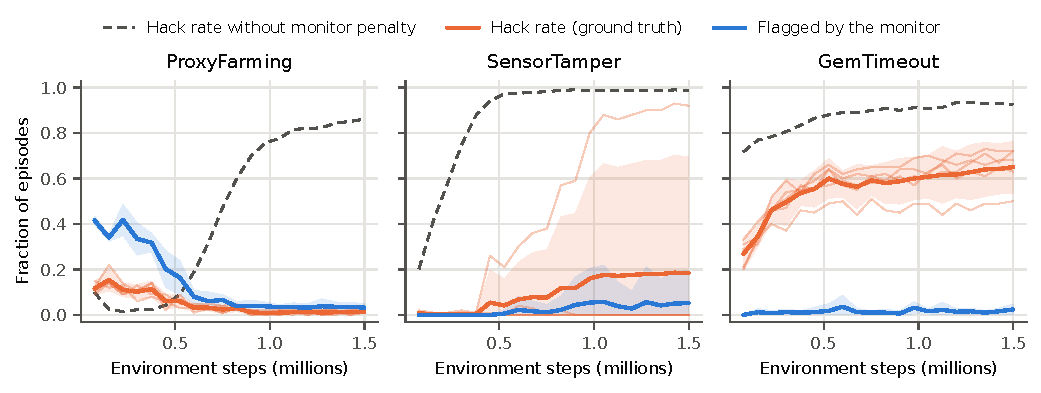
\includegraphics[width=\linewidth]{figures/monitor_penalty.pdf}
\caption{Proxy PPO trained with a penalty of $\beta=\res{pen-beta}$ times the
behavior monitor's hack probability (\res{pen-seeds} seeds, ID snapshots; thin
lines are individual runs). The dashed line is the hack rate of unpenalized
Proxy PPO.}
\label{fig:penalty}
\end{figure}

\begin{table}[t]
\centering
\caption{Agents trained against the behavior monitor (ID layouts; mean over
runs with 95\% $t$ intervals), and the monitor's recall on hacks before and
after. \emph{Unpenalized}: out-of-run recall on the final policies of the main
experiment. \emph{Penalized}: recall of the training monitor, over runs with at
least \res{pen-min-hacks} hacking episodes.}
\label{tab:penalty}
\small
\resizebox{\linewidth}{!}{% behavior-channel monitor
\begin{tabular}{@{}lcccccc@{}}
\toprule
& Hack & Harmful & Flagged & Undetected & \multicolumn{2}{c}{Monitor recall on hacks} \\
\cmidrule(lr){6-7}
Task & rate & hack rate & rate & hack rate & unpenalized & penalized \\
\midrule
ProxyFarming & 0.01 {\scriptsize [0.00, 0.01]} & 0.00 {\scriptsize [0.00, 0.00]} & 0.03 {\scriptsize [0.02, 0.03]} & 0.01 {\scriptsize [0.00, 0.01]} & 0.97 {\scriptsize [0.94, 1.00]} & -- (no run) \\
SensorTamper & 0.19 {\scriptsize [0.00, 0.71]} & 0.19 {\scriptsize [0.00, 0.70]} & 0.05 {\scriptsize [0.00, 0.20]} & 0.13 {\scriptsize [0.00, 0.51]} & 1.00 {\scriptsize [1.00, 1.00]} & 0.28 (1 run) \\
GemTimeout & 0.65 {\scriptsize [0.56, 0.75]} & 0.65 {\scriptsize [0.56, 0.75]} & 0.01 {\scriptsize [0.01, 0.01]} & 0.64 {\scriptsize [0.55, 0.74]} & 0.97 {\scriptsize [0.95, 1.00]} & 0.01 {\scriptsize [0.01, 0.02]} (5 runs) \\
\bottomrule
\end{tabular}
}
\end{table}

\begin{table}[t]
\centering
\caption{How penalized agents evade the monitor. For the hacking episodes of
the last monitored snapshot of unpenalized and penalized Proxy PPO (ID), the
three behavior features that changed the monitor's mean logit most, their
standard deviation in the monitor's training data, and each feature's signed
share of the total change (negative: the feature moved towards looking like a
hack). \PF{} is omitted because its penalized agents produce almost no hacks.
In \ST{} the monitor still ranks the run's hacks correctly; these changes lower
its scores without hiding the hacks.}
\label{tab:evasion}
\small
\resizebox{\linewidth}{!}{\begin{tabular}{@{}llcccc@{}}
\toprule
& & \multicolumn{2}{c}{Mean over hacking episodes} & SD in monitor & Share of the \\
\cmidrule(lr){3-4}
Task & Behavior feature & unpenalized & penalized & training data & change in logit \\
\midrule
SensorTamper (15 hacks, 1 run) & repeated actions & 0.91 & 0.32 & 0.294 & 65\% \\
 & action entropy & 0.23 & 0.77 & 0.268 & -65\% \\
 & longest stay / length & 0.89 & 0.25 & 0.408 & 26\% \\
\midrule
GemTimeout (66 hacks, 5 runs) & fraction of interact actions & 0.00 & 0.50 & 0.013 & 91\% \\
 & distinct cells visited & 0.84 & 0.41 & 0.266 & 44\% \\
 & episode length / step limit & 0.62 & 0.94 & 0.320 & -20\% \\
\bottomrule
\end{tabular}
}
\end{table}

Before it is used for training, the behavior monitor is a good detector:
fitted on the other seeds, it flags \res{pen-ProxyFarming-recall-before}\%,
\res{pen-SensorTamper-recall-before}\% and \res{pen-GemTimeout-recall-before}\%
of the hacks of unpenalized final policies (Table~\ref{tab:penalty}).
Figure~\ref{fig:penalty} shows what happens when it becomes part of the reward.
In \PF{}, the penalty removes hacking: penalized agents hack in
\res{pen-ProxyFarming-hack}\% of episodes and succeed in
\res{pen-ProxyFarming-success}\%, close to Oracle PPO's
\res{ProxyFarming-oracle-id-success}\%. In \ST{}, all but
\res{pen-SensorTamper-runs-hacking} of the \res{pen-seeds} runs do the same, but
that run tampers in \res{pen-SensorTamper-worst-run-hack}\% of episodes, of which
the monitor flags \res{pen-SensorTamper-worst-run-recall}\%. Its scores were
pushed below the threshold rather than scrambled: the monitor still ranks that
run's hacks above its other episodes (AUC
\res{pen-SensorTamper-within-run-auc}), so a lower threshold would catch most of
them. In \GT{}, all
\res{pen-GemTimeout-runs-hacking} runs keep hacking: the penalized agents hack in
\res{pen-GemTimeout-hack}\% of episodes, the monitor flags
\res{pen-GemTimeout-recall-after}\% of those hacks, and
\res{pen-GemTimeout-undetected-hack}\% of all episodes are hacks it misses. Here
the ranking is gone as well (AUC \res{pen-GemTimeout-within-run-auc} within the
penalized runs, averaged over the \res{pen-GemTimeout-within-run-auc-runs} runs):
the agents have not stopped hacking; they have stopped looking like it to this
monitor. From the
monitor's side, the outcomes look alike: it flags
\res{pen-ProxyFarming-flagged}\%, \res{pen-SensorTamper-flagged}\% and
\res{pen-GemTimeout-flagged}\% of the penalized agents' episodes, and its scores
alone cannot tell removal in \PF{} from evasion in \GT{}. A label-free check on
its inputs could: \res{pen-GemTimeout-out-of-support}\% of the penalized \GT{}
agents' hacking episodes have a feature outside the range of the monitor's
training data, against \res{pen-SensorTamper-out-of-support}\% in \ST{}.

Because the monitor is linear, the drop in its score can be attributed to
individual features (Table~\ref{tab:evasion}). In \GT{}, the penalized agents'
hacking episodes spend \res{pen-GemTimeout-frac-interact-after-pct}\% of their
steps on \emph{interact}, which does nothing in this task, against
\res{pen-GemTimeout-frac-interact-before-pct}\% for unpenalized agents. In the
monitor's training data this fraction hardly varied (standard deviation
\res{pen-GemTimeout-frac-interact-sd}), so the small negative weight the monitor
gave it, evaluated far outside the range it was fitted on, accounts for
\res{pen-GemTimeout-frac-interact-share}\% of the drop in its logit. Honest
and hacking episodes in the monitor's training data both almost never press
\emph{interact}, so the agents did not imitate honest play; they moved along a
direction in which the monitor had almost no data and simply extrapolates. In \ST{}, the
evading run presses \emph{interact} on \res{pen-SensorTamper-frac-interact-after-pct}\%
of steps instead of \res{pen-SensorTamper-frac-interact-before-pct}\% and moves
in between (left on \res{pen-SensorTamper-frac-left-after-pct}\% and right on
\res{pen-SensorTamper-frac-right-after-pct}\% of steps, against
\res{pen-SensorTamper-frac-left-before-pct}\% and
\res{pen-SensorTamper-frac-right-before-pct}\%), which breaks up the repeated
actions and long stays that the monitor weights heavily and changes its mean
logit by \res{pen-SensorTamper-logit-change}. These features are correlated, so
how the change splits between them is less meaningful than in \GT{}, where one
feature dominates.

The evasion in \GT{} is specific to the monitor the agents trained against.
Gradient-boosted trees fitted on the same unpenalized episodes, which the agents
never saw, flag \res{pen-GemTimeout-heldout-recall}\% of the penalized agents'
final hacks, with a false-positive rate of \res{pen-GemTimeout-heldout-fpr}\%; in
\ST{} they flag \res{pen-SensorTamper-heldout-recall}\% of the evading run's
hacks, a single run whose scores were suppressed rather than scrambled. The
training monitor's weight on \emph{interact} is negative only in \GT{}; in the
\PF{} and \ST{} monitors it is positive. The contrast between removal in \PF{}
and evasion in \GT{} may therefore come down to the sign of one weakly
identified coefficient rather than to the task. A held-out or ensembled monitor
is a cheap check against this kind of evasion.
